\part{X-ray Simulation using QMC Methods}

\chapter{Motivation and Problem Statement} % Main chapter title
\label{Chapter6}


%-------------------------------------------------------------------------------
%	SECTION 1
\section{Computed Tomography Imaging}
%-------------------------------------------------------------------------------

\ac{ct} imaging is a powerful medical imaging technique that provides detailed
cross-sectional images of the body by combining multiple X-ray projections taken
from different angles. This technique is widely used for diagnostic purposes,
allowing clinicians to visualize internal structures with high spatial
resolution.

The process involves rotating an X-ray source around the patient while
simultaneously capturing X-ray projections on a detector array. Each projection
represents the cumulative attenuation of X-rays as they pass through various
tissues, influenced by the density and composition of the materials they
encounter.

The collected data is then reconstructed into a three-dimensional volume
using advanced algorithms, such as filtered backprojection or iterative
reconstruction methods. These algorithms convert the raw projection data into
cross-sectional images, which can be further processed to enhance contrast,
reduce noise, and improve overall image quality.

To achieve accurate reconstructions, it is crucial to acquire high-quality X-ray
projection images. However, one of the most significant challenges in CT imaging
is the presence of scattered radiation - such as Comton and Rayleigh scattering
- which can lead to artifacts and distortions in the reconstructed images.

Throughout this thesis, the term \textit{scatter reduction in \ac{ct}} refers to
the mitigation of scatter-induced artifacts in the two-dimensional X-ray
projection images acquired by the detector array during a CT scan. These
projections serve as the input for reconstructing the final three-dimensional
volume. Given the complexity of the full reconstruction process, the focus of
this work is limited to analyzing and correcting scatter effects at the level of
the two-dimensional projection data.


%-------------------------------------------------------------------------------
%	SECTION 2
\section{X-ray Imaging and the Challenge of Scatter}
%-------------------------------------------------------------------------------

X-ray \ac{ct} relies on measuring the attenuation of X-rays along straight-line
paths through a phantom. Here, the X-ray beam is further abstracted as
individual photons with defined initial energies and directions. The photon
trajectories typically extend from an X-ray source $\mathcal{S}$ to a detector
element $\mathcal{D}$, forming the path:

$$l = \overrightarrow{\mathcal{S}\mathcal{D}}$$

Under idealized conditions, the attenuation process is governed by the
\emph{Lambert-Beer law}, which describes an exponential decay in intensity $I$
as the beam interacts with the material. As stated in
\cite[Chap.~7]{medicalImagingSystemsIntro2019:}, this relationship is given by:

\begin{equation}
    \label{eq:lambert_beer_law}
     I = I_0(E)\cdot \int_0^{E_\text{max}} \exp\bigg(-\int_{{\mathcal{S}}}^{\mathcal{D}} \mu(x,E) \, dx\bigg) \, dE
\end{equation}

Here, $I_0(E)$ denotes the incident intensity of X-rays with initial energy $E$
at the source $\mathcal{S}$, and $\mu(x,E)$ represents the linear attenuation
coefficient at spatial location $x$ along the path $l$, for energy $E$. The
resulting intensity $I$ is measured at the detector element $\mathcal{D}$.

Although exponential attenuation along straight-line paths such as
$\overrightarrow{\mathcal{S}\mathcal{D}}$ is the idealized model for X-ray
imaging, this assumption is systematically violated in practice. As X-rays
traverse the scanned phantom, many photons undergo scattering interactions -
such as Compton or Rayleigh scattering - that alter their trajectories. Despite
deviating from the primary path, these scattered photons may still reach the
detector, adding unintended signal components. As a result, the measured
intensities no longer represent pure line integrals of the attenuation map. This
discrepancy introduces nonlinear errors and visible artifacts in the
reconstructed image, ultimately degrading both visual quality and quantitative
accuracy.

Scattered radiation is a major source of image artifacts - such as cupping and
streaks - and reduces both spatial and contrast resolution. These effects not
only degrade visual image quality but also compromise the accuracy of
quantitative measurements, such as Hounsfield units $\mu_*$, which are used for
clinical interpretation, such as tissue characterization
\cite[Chap.~8]{medicalImagingSystemsIntro2019:}. Hounsfield units represent a
normalized attenuation relative to the attenuation of water:

\begin{equation}
    \mu_* = \left(\frac{\mu}{\mu_{\text{water}}} -1\right) \cdot 1000
\end{equation}

The impact of scatter becomes especially pronounced in modern CT systems using
high-energy X-rays or large-area flat-panel detectors, where scatter may
dominate the measured signal. As such, accurate modeling and correction of
scatter are essential for achieving high-fidelity CT images, particularly in
clinical applications where precision and reliability are paramount
\citep{medicalImagingSystemsIntro2019:}.


%-------------------------------------------------------------------------------
%	SECTION 3
\section{Scatter Correction Methods for X-ray Imaging}
%-------------------------------------------------------------------------------

\subsection{Overview of Scatter Correction Techniques}

In X-ray imaging, scattered photons are a major source of image artifacts and
quantitative inaccuracies. To mitigate these effects, a range of computational
scatter correction methods has been developed. These approaches can be broadly
classified into the following categories:

\begin{itemize}
    \item \textbf{Empirical and Analytical Methods:} \\
        These include techniques such as primary modulation, convolution-based
        correction, and energy windowing. Scatter is typically estimated using
        simplified models or empirical kernels, often assuming a smooth
        background distribution, and then subtracted from the measured signal.
        While computationally efficient, these methods rely on assumptions
        regarding the spatial and energy distribution of scattered photons. As a
        result, they may fail to accurately model complex scatter phenomena in
        heterogeneous anatomical structures.

    \item \textbf{Physics-Based Models:} \\
        These methods aim to provide a more accurate representation of the
        underlying photon transport physics, including scattering phenomena.
        Among them, \ac{mc} simulation is regarded as the most rigorous and
        comprehensive technique due to its ability to statistically model
        complex photon interactions without relying on simplifying assumptions.
        In such simulations, primary and scattered photon contributions are
        detected separately, allowing the estimated scatter signal to be
        subtracted from measured data in order to restore image fidelity.
\end{itemize}

In \citeyear{mcffd2011}, \citeauthor{mcffd2011} \cite{mcffd2011} already
demonstrated promising results using computationally expensive \ac{mc}
simulations of CT scans of a cylindrical phantom with two bone inserts. The
results showed significant improvements in image quality, as illustrated by
\citeauthor{mcffd2011} in Figure~\ref{fig:scatter_correction_comparison}.

\captionsetup{justification=justified,singlelinecheck=false}
\begin{figure}[H]
    \centering
    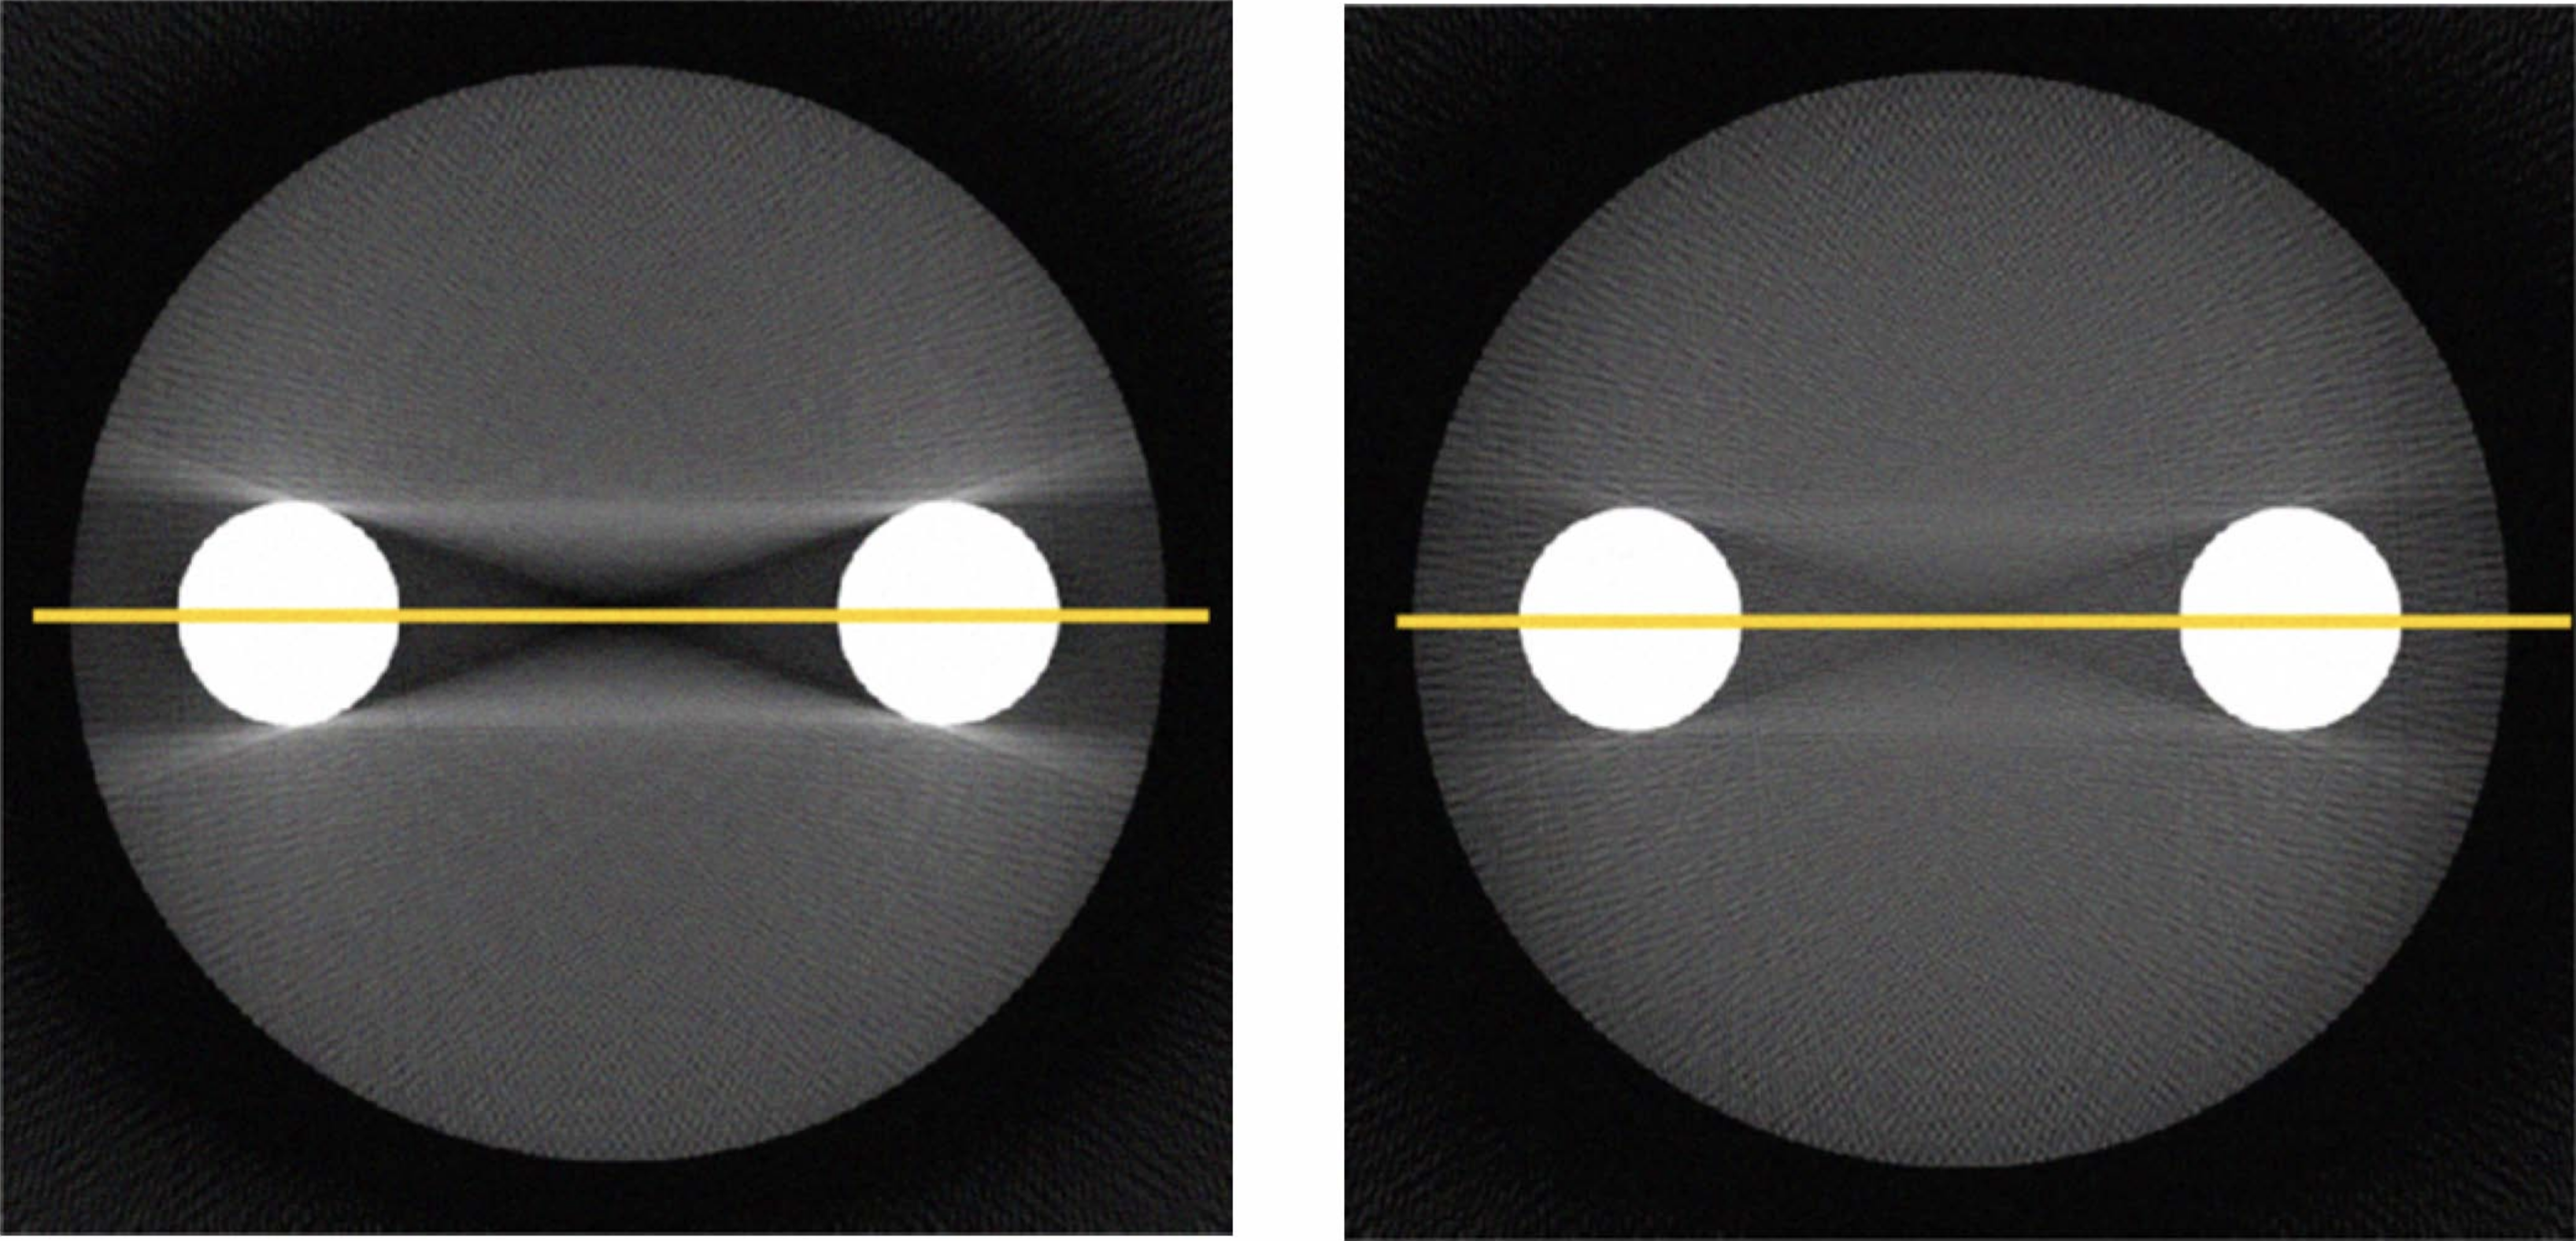
\includegraphics[width=0.8\textwidth]{Figures/mcffd.png}
    \caption{\ac{cbct} of a 70\,mm soft-tissue cylinder with two bone inserts.
    Right: Simulation of a X-ray image with scattering, exibiting typical
    cupping and streak artifacts. Right: Image after scatter correction applying
    \ac{mc} techniques for the simulation of $5 \times 10^6$ photons, showing
    improved uniformity and quantitative accuracy. Right: Image without
    correction, exhibiting typical cupping and streak artifacts. (Figure adapted from \cite{mcffd2011}, \textcopyright 2011 IEEE)}
    \label{fig:scatter_correction_comparison}
\end{figure}


\subsection{Monte Carlo Simulation}

To achieve scatter correction using \ac{mc} simulation, a three-dimensional
phantom is first estimated by analyzing the X-ray projections. Then, an
\ac{mc} simulation is performed to estimate the scatter signal
$I_\text{scattered}$ for each detector pixel. This estimated scatter signal is
then subtracted from the measured intensity $I_\text{measured}$:

\begin{equation}
    \label{eq:scatter_correction}
    I_{\text{corrected}} = I_\text{measured} - I_\text{scattered}
\end{equation}

The \ac{mc} simulation is a powerful computational technique that follows
physics-based principles to model the transport of photons through matter. It is
widely recognized as the gold standard for scatter correction in CT and related
imaging modalities. This status is attributed to several key factors:

\begin{itemize}
    \item \textbf{Physical Accuracy:} \\
        \ac{mc} methods simulate the stochastic nature of photon interactions -
        including Compton and Rayleigh scattering, photoelectric absorption, and
        multiple scattering events - based on fundamental physical
        cross-sections and material properties.

    \item \textbf{Comprehensive Modeling:} \\
        Unlike analytical or empirical methods, \ac{mc} simulations can account
        for complex geometries, heterogeneous materials and realistic X-ray
        spectra, providing highly accurate estimates of the scatter signal.

    \item \textbf{Validation Benchmark:} \\
        Due to their accuracy, \ac{mc}-based scatter estimates are routinely
        used as reference standards for validating and benchmarking faster,
        approximate correction methods.
\end{itemize}


%-------------------------------------------------------------------------------
%	SECTION 4
\section{High-Level Overview of the Monte Carlo Simulation}
%-------------------------------------------------------------------------------

The \ac{mc} simulation of photon transport for scatter correction typically involves the following key steps \cite{mcffd2011}:

\begin{enumerate}
    \item \textbf{Photon Emission:} \\
        Photons are emitted from a virtual X-ray source, with their energies sampled
        from a predefined source spectrum.
        
    \item \textbf{Photon Tracking:} \\
        Each photon is tracked as it propagates through the object. At every
        step, the probability of interaction (either scattering or absorption)
        is determined by the local material properties and corresponding
        interaction cross-sections.
        
    \item \textbf{Interaction Sampling:} \\
        Upon interaction, the event type (e.g., Compton scattering, Rayleigh
        scattering, or photoelectric absorption) and the resulting change in
        photon direction and energy are sampled from the relevant probability
        distributions.
        
    \item \textbf{Detection:} \\
        Photons that reach the detector—either unscattered or after one or more
        scattering events—are recorded. The simulation distinguishes between
        primary and scattered photons, thereby enabling an accurate estimation
        of the scatter contribution at each detector element.
        
    \item \textbf{Statistical Averaging:} \\
        By simulating a large number of photons, the method builds a
        statistically robust estimate of the scatter distribution. The accuracy
        of the result increases with the number of simulated photons and
        ultimately converges toward a stable intensity distribution.
\end{enumerate}

The schematic flow of the Monte Carlo simulation process is summarized in
Figure~\ref{fig:photon-transport-pseudocode}.

\begin{figure}[H]
\centering
\begin{tcolorbox}[colback=white!95!gray, colframe=black!60, width=0.9\textwidth, title=Monte Carlo Photon Transport Algorithm, fonttitle=\bfseries]
\begin{itemize}[leftmargin=1.5em]
    \item \textbf{Initialization:} Define geometry, material composition, and source
    spectrum.
    
    \item \textbf{Loop over photons:}
    \begin{itemize}
        \item Sample the step size to the next interaction point.
        \item Move the photon; check for boundary crossings.
        \item Sample the interaction type; update direction and energy.
        \item If the photon reaches the detector, record the event.
        \item If the photon is absorbed or exits the system, terminate its trajectory.
    \end{itemize}
    
    \item \textbf{Aggregation:} Compute both scatter and primary intensity distributions.
\end{itemize}
\end{tcolorbox}
\caption{Pseudocode representation of the Monte Carlo algorithm for photon transport in scatter modeling.}
\label{fig:photon-transport-pseudocode}
\end{figure}


%-------------------------------------------------------------------------------
%SECTION 5
\section{Monte Carlo Methods: Benefits \& Drawbacks}
%-------------------------------------------------------------------------------

\ac{mc} simulations are widely regarded as the gold standard for scatter
correction in computed tomography due to their ability to model photon-matter
interactions from first principles. These simulations accurately reproduce all
relevant physical scattering phenomena - including Compton and Rayleigh
scattering - and can accommodate arbitrarily complex geometries and
heterogeneous material compositions. Owing to this high degree of physical
fidelity, MC-based methods yield highly accurate scatter estimates and are
commonly employed as reference standards for evaluating and validating
alternative correction approaches.

However, the high accuracy of Monte Carlo simulations comes at the cost of
substantial computational effort. Producing low-noise scatter estimates requires
the simulation of a large number of photon histories to ensure statistical
convergence. Consequently, the runtime scales with the desired level of
accuracy and may range from several minutes to multiple hours or even days,
depending on the complexity of the scene and the available computational
resources. This computational burden poses a major limitation, particularly in
applications involving large datasets or iterative reconstruction workflows.

To address the computational inefficiency of slow-converging \ac{mc}
methods, recent research has explored strategies to accelerate physically
accurate photon transport simulations. Among these, the application of
\ac{qmc} methods has gained increasing attention. By replacing random sampling
with deterministic low-discrepancy sequences, \ac{qmc} techniques can achieve
significantly faster convergence while maintaining comparable accuracy.
Recent \ac{qmc}-based scatter correction algorithms have demonstrated runtime
reductions of multiple orders of magnitude, thereby enabling high-fidelity
simulations even in time-sensitive or resource-constrained environments
\cite{qmcXray2023,lin2025scatter, doignies2024echantillonnage}.
